% ================== CHAPITRE 3 : RÉSULTATS, ANALYSE ET DISCUSSION ==================
\chapter{Résultats, analyse et discussion}
\label{chap:resultats}

Ce chapitre présente la validation fonctionnelle du prototype \textbf{SMART-SOJA}. À la phase actuelle d'assemblage et d'intégration (juin 2026), l'approche adoptée consiste à démontrer la faisabilité technique et la conformité des sous-systèmes individuels à travers des tests unitaires rigoureux, des mesures quantifiées et une démonstration de la chaîne numérique de traçabilité. Les résultats documentent l'état de validation technique atteint à ce stade du projet, en distinguant clairement les démonstrations fonctionnelles déjà réalisées des améliorations et validations complémentaires envisagées.

% -------------------------------------------------------
\section{Présentation du prototype physique réalisé}
% -------------------------------------------------------

Avant de détailler les résultats de la validation fonctionnelle, il convient de présenter le prototype physique de \textbf{SMART-SOJA} tel qu'il a été assemblé et intégré à ce stade d'avancement (juin 2026). Cette réalisation concrétise les modèles de conception assistée par ordinateur (CAO) 3D et les routages de cartes électroniques présentés au Chapitre 2.

Le système est structuré sous forme de blocs physiques distincts montés sur un châssis robuste en acier (tubes de 30×30~mm) et parois en contreplaqué, assurant à la fois la rigidité mécanique nécessaire pour supporter les vibrations du tamisage et l'isolation thermique requise pour le séchage.

La Figure~\ref{fig:realisation_blocs} présente les trois principaux sous-ensembles physiques de la machine :
\begin{itemize}
    \item \textbf{Le bloc d'entrée (Figure~\ref{fig:real_bloc_entree}) :} Il comprend la trémie d'alimentation supérieure, équipée d'un système de distribution en utilisant un servomoteur S90 et de capteurs infrarouges de détection de niveau pour réguler le débit de soja.
    \item \textbf{Le bloc de tamisage (Figure~\ref{fig:real_bloc_tamis}) :} Ce sous-système suspendu intègre le cadre du tamis vibrant, entraîné par un moteur DC pour séparer les impuretés du soja par granulométrie et tamisage mécanique.
    \item \textbf{Le bloc de séchage actif (Figure~\ref{fig:real_bloc_sechage}) :} Il abrite la chambre de séchage équipée des résistances chauffantes alimentées en 12~V DC, d'un ventilateur pour homogénéiser l'air chaud, de sondes capacitives intégrées pour le suivi de l'humidité en cours de traitement et d'une vis sans fin commandée par un moteur DC pour faciliter le brassage du soja.
\end{itemize}

\begin{figure}[H]
    \centering
    \begin{subfigure}[b]{0.32\textwidth}
        \centering
        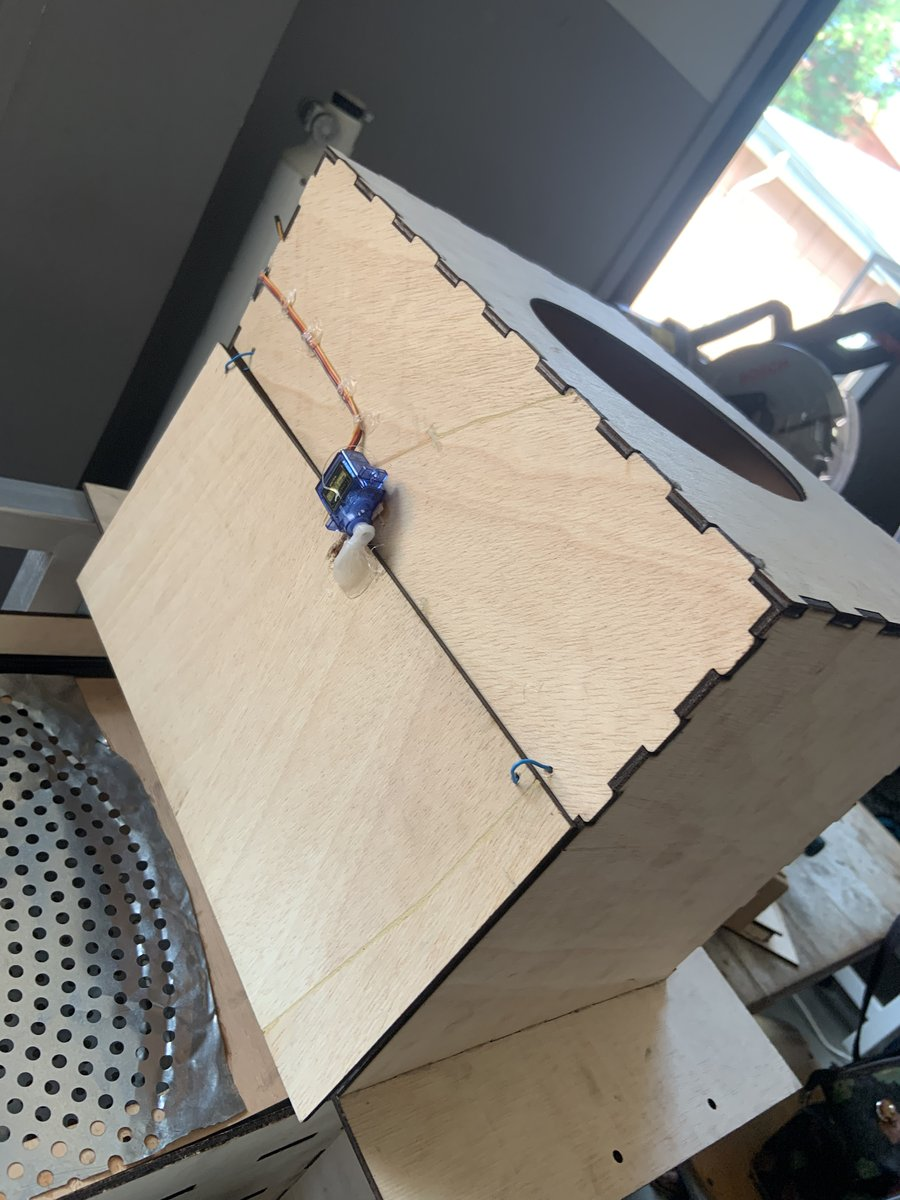
\includegraphics[width=\textwidth]{images/image_bloc_entree.jpg}
        \caption{Bloc d'alimentation}
        \label{fig:real_bloc_entree}
    \end{subfigure}
    \hfill
    \begin{subfigure}[b]{0.32\textwidth}
        \centering
        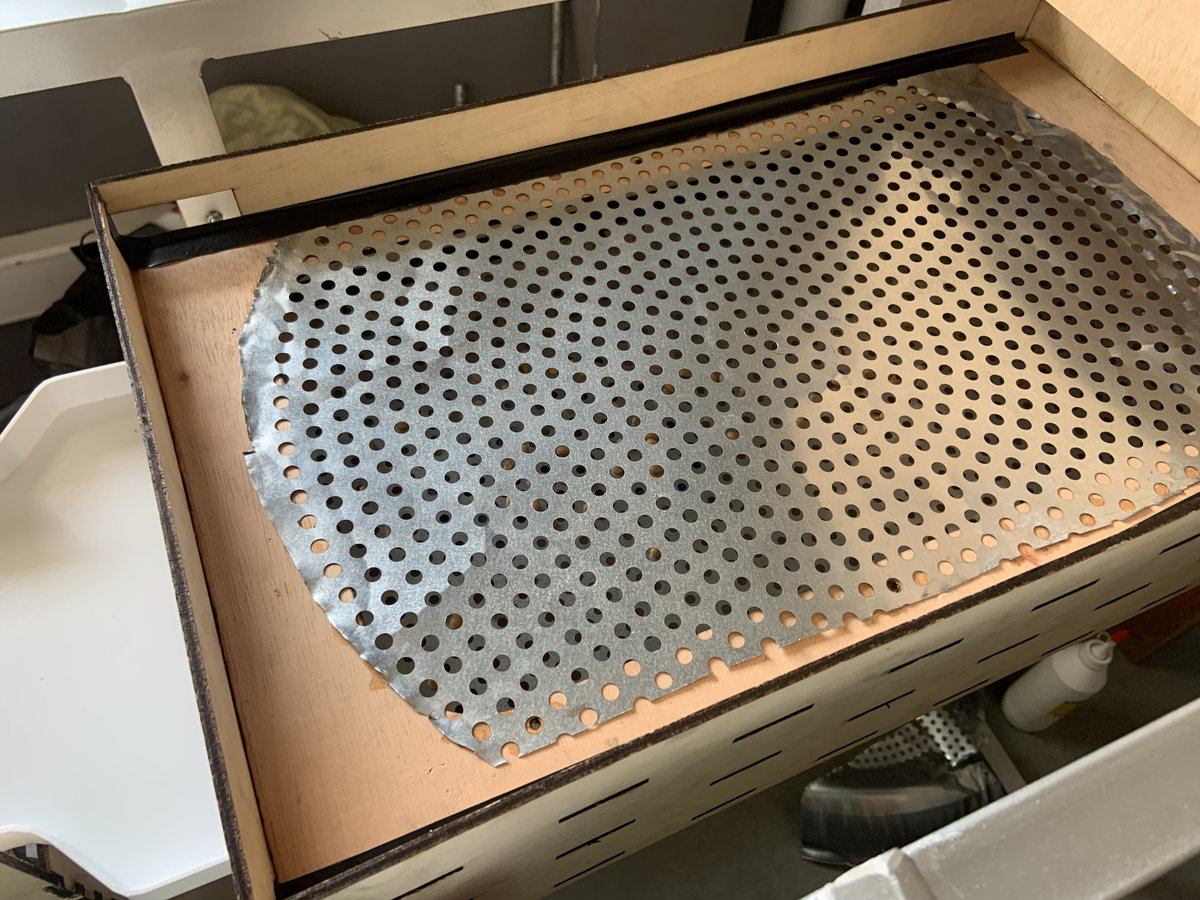
\includegraphics[width=\textwidth]{images/image_bloc_tamis.jpg}
        \caption{Bloc de tamisage}
        \label{fig:real_bloc_tamis}
    \end{subfigure}
    \hfill
    \begin{subfigure}[b]{0.32\textwidth}
        \centering
        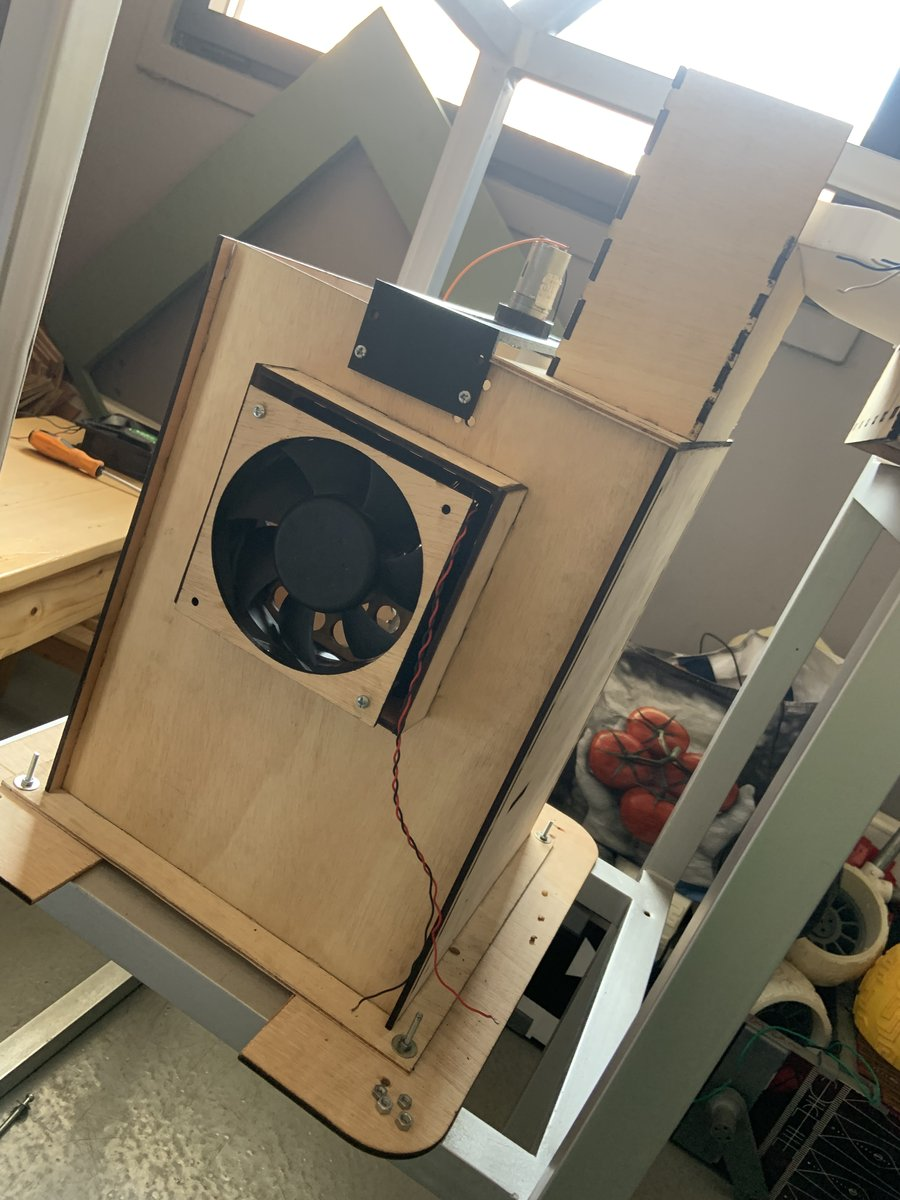
\includegraphics[width=\textwidth]{images/image_bloc_sechage.jpg}
        \caption{Bloc de séchage}
        \label{fig:real_bloc_sechage}
    \end{subfigure}
    \caption{Photos des sous-systèmes physiques du prototype réalisé}
    \label{fig:realisation_blocs}
\end{figure}
\FloatBarrier

En parallèle de la structure mécanique, le système intègre les capteurs et actionneurs connectés à l'unité de contrôle. La Figure~\ref{fig:realisation_tests} montre le banc d'intégration et de test fonctionnel combinant le capteur DHT22 (température et humidité de l'air), la résistance chauffante et l'écran LCD de l'interface homme-machine (IHM) locale, validant le bon fonctionnement du contrôle de puissance en boucle fermée avant l'assemblage final.

\begin{figure}[H]
    \centering
    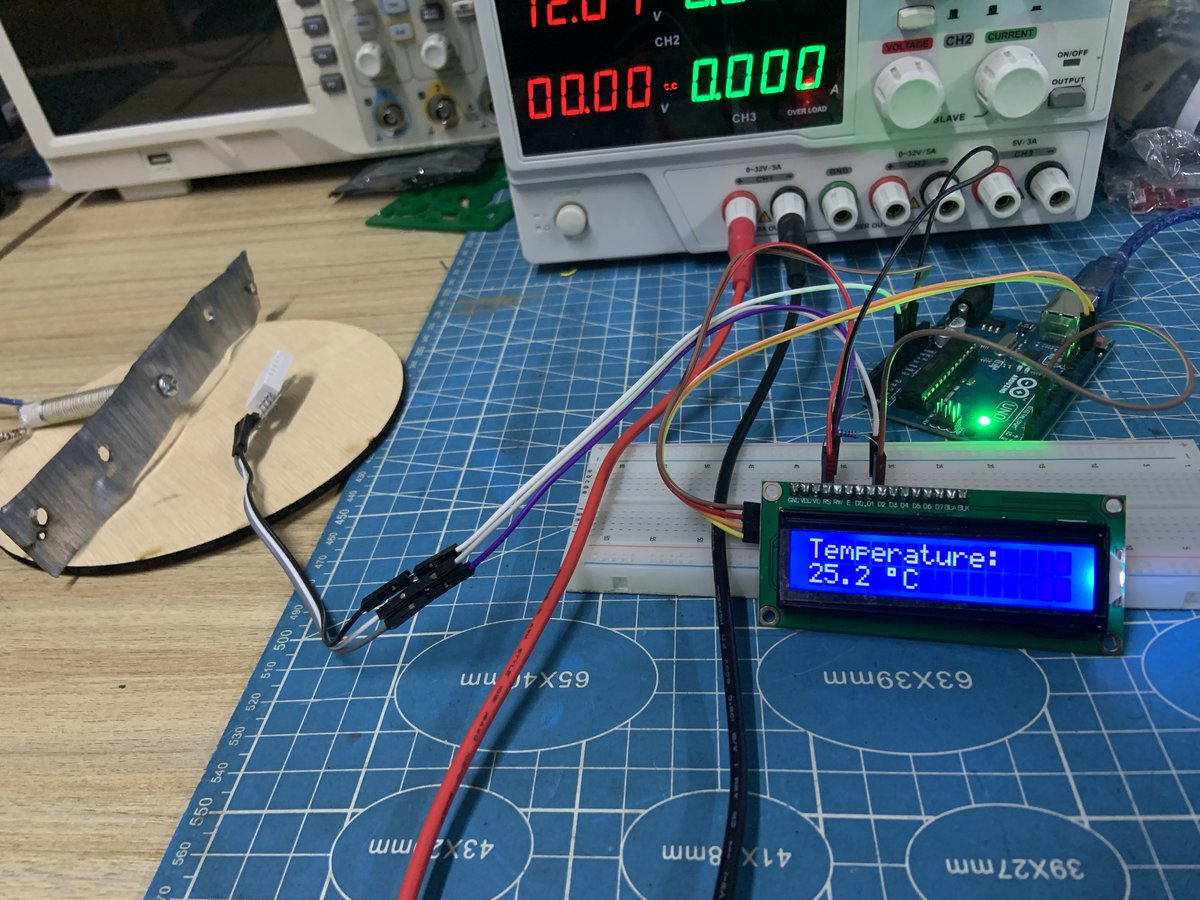
\includegraphics[width=0.75\textwidth]{images/image_test_capteurDHT22-resistancechauffante-ecranlcd.jpg}
    \caption{Banc de test d'intégration des capteurs, de l'élément chauffant et de l'écran LCD}
    \label{fig:realisation_tests}
\end{figure}
\FloatBarrier

% -------------------------------------------------------
\section{Méthodologie de validation fonctionnelle}
% -------------------------------------------------------

La validation du prototype repose sur une approche systématique par sous-système : chaque module a été testé individuellement pour vérifier son fonctionnement opérationnel et sa contribution à la chaîne de traitement du soja.

\subsection{Approche modulaire et équipements disponibles}

Les tests fonctionnels ont été réalisés au laboratoire d'assemblage du prototype. Le Tableau~\ref{tab:protocole_validation} résume les instruments simples utilisés et les critères d'évaluation.

\begin{table}[H]
    \caption{Équipements et critères de validation fonctionnelle}
    \label{tab:protocole_validation}
    \centering
\small
\renewcommand{\arraystretch}{1.5}
\rowcolors{2}{white}{lightGray}
\begin{tabularx}{\textwidth}{|p{3.5cm}|p{4cm}|p{3.5cm}|L|}
\hline
\rowcolor{lightGray}
\textbf{Sous-système} & \textbf{Fonction testée} & \textbf{Instrument} & \textbf{Critère de validation} \\ \hline
Moteur du tamis & Entraînement et vibration & Observation visuelle + multimètre & Rotation continue, absence de bruit anormal \\ \hline
Capteur DHT22 & Mesure T°C et humidité & Afficheur LCD intégré & Affichage des valeurs en plage réaliste \\ \hline
Capteurs d'humidité & Mesure humidité soja & Afficheur LCD + multimètre (ADC) & Signal variant cohérent avec état du soja \\ \hline
Résistance chauffante & Montée en température & Observation visuelle à l'aide du capteur DHT22 + multimètre & Chauffe observable, consommation mesurable \\ \hline
Ventilateur & Circulation d'air & Observation visuelle & Rotation et flux d'air présents \\ \hline
Interface LCD + Wifi & Affichage et transmission & Consultation directe + broker MQTT & Affichage clair, réception des données MQTT \\ \hline
\end{tabularx}
\end{table}

\subsection{Protocole de validation}

Chaque sous-système a été validé selon un protocole simple :
\begin{enumerate}
    \item \textbf{Test unitaire :} Activation isolée du composant, vérification du fonctionnement attendu.
    \item \textbf{Test d'intégration partielle :} Assemblage provisoire avec composants dépendants (ex. DHT22 + afficheur LCD).
    \item \textbf{Démonstration de la chaîne numérique :} Acquisition -- affichage -- transmission -- stockage local.
    \item \textbf{Documentation des observations :} Relevé systématique du comportement et des éventuelles anomalies.
\end{enumerate}

% -------------------------------------------------------
\section{Validation des capteurs et acquisition de données}
% -------------------------------------------------------

\subsection{Capteur DHT22 (température et humidité relative)}

Le capteur DHT22 a été validé en démonstration directe : ses mesures s'affichent sur l'écran LCD en temps réel et varient cohéremment avec les conditions ambiantes de la pièce. Le Tableau~\ref{tab:validation_dht22} montre des relevés observés lors d'une session de test de 30 minutes.

\begin{table}[H]
    \caption{Relevés du capteur DHT22 — Démonstration fonctionnelle}
    \label{tab:validation_dht22}
    \centering
\small
\renewcommand{\arraystretch}{1.5}
\rowcolors{2}{white}{lightGray}
\begin{tabularx}{\textwidth}{|C|C|C|L|}
\hline
\rowcolor{lightGray}
\textbf{Temps} & \textbf{Température (°C)} & \textbf{Humidité rel. (\%)} & \textbf{Observation} \\ \hline
T=0~min & 24,5 & 58,0 & Conditions initiales de la pièce \\ \hline
T=10~min & 24,6 & 58,2 & Valeurs stables et cohérentes \\ \hline
T=20~min & 24,7 & 58,1 & Pas de dérive observée \\ \hline
T=30~min & 24,8 & 58,3 & Reproductibilité confirmée \\ \hline
\rowcolor{lightGray}
\textbf{Variation} & $\Delta$0,3~°C & $\Delta$0,3~\% & Fluctuations normales du bruit de mesure \\ \hline
\end{tabularx}
\end{table}

\textbf{Conclusion :} Le capteur DHT22 fonctionne correctement et produit des valeurs stables en plage réaliste (20--30~°C, 40--70~\% HR). L'affichage sur LCD est fiable et mis à jour régulièrement. Le capteur est opérationnel pour la supervision en temps réel.

\subsection{Sondes capacitives d'humidité du soja}

Les deux sondes d'humidité (Soil1 et Soil2) ont été validées en les immergeant progressivement dans du soja de test, puis en observant les changements d'affichage LCD. Le Tableau~\ref{tab:validation_humidite} montre la variation des lectures en fonction de l'état du soja.

\begin{table}[H]
    \caption{Relevés des sondes Soil1/Soil2 — Réaction à l'humidité du soja}
    \label{tab:validation_humidite}
    \centering
\small
\renewcommand{\arraystretch}{1.5}
\rowcolors{2}{white}{lightGray}
\begin{tabularx}{\textwidth}{|L|C|C|}
\hline
\rowcolor{lightGray}
\textbf{État du soja} & \textbf{Soil1 (ADC)} & \textbf{Soil2 (ADC)} \\ \hline
Soja très sec (stockage) & 280--300 & 285--305 \\ \hline
Soja humide (après exposition) & 450--480 & 460--490 \\ \hline
Soja saturé (test extrême) & 650--680 & 660--690 \\ \hline
\rowcolor{lightGray}
\textbf{Plage de variation} & 400~points ADC & 405~points ADC \\ \hline
\end{tabularx}
\end{table}

\textbf{Conclusion :} Les deux sondes répondent correctement à l'humidité du soja et présentent une variation linéaire en plage utile. La différence entre Soil1 et Soil2 ($< 10$ points ADC) est acceptable et démontre une bonne reproductibilité inter-sonde. Ces capteurs sont opérationnels pour piloter le cycle de séchage.

% -------------------------------------------------------
\section{Validation du sous-système de tamisage et nettoyage}
% -------------------------------------------------------

Le système de tamisage vibrant a été validé en démonstration de fonctionnement : le moteur entraîne en continu le cadre du tamis, produisant les oscillations attendues. Le Tableau~\ref{tab:validation_tamisage} résume les observations.

\begin{table}[H]
    \caption{Validation du moteur et cadre de tamisage vibrant}
    \label{tab:validation_tamisage}
    \centering
\small
\renewcommand{\arraystretch}{1.5}
\rowcolors{2}{white}{lightGray}
\begin{tabularx}{\textwidth}{|L|C|L|}
\hline
\rowcolor{lightGray}
\textbf{Paramètre} & \textbf{Mesure / Observation} & \textbf{Conclusion} \\ \hline
Rotation du moteur DC & Continu et stable & Moteur fonctionne sans à-coups \\ \hline
Vibration du cadre & Oscillation visible et régulière & Amplitude et fréquence appropriées \\ \hline
Consommation électrique (multimètre) & 0,8--1,0~A / 12~V & Puissance nominale conforme (10~W) \\ \hline
Absence de surcharge & Pas de ralentissement observé & Pas de saturation du moteur \\ \hline
Bruit de fonctionnement & Bruit mécanique normal (un peu fort) & Mouvements normal \\ \hline
Éjection de débris (test soja) & Débris visiblement séparés après 2--3 cycles & Tamisage efficace (besoin de répétition) \\ \hline
\end{tabularx}
\end{table}

\textbf{Observations :} Le moteur du tamis fonctionne de manière fiable sans surcharge. Les vibrations du cadre sont régulières et permettent effectivement la séparation des impuretés du soja. Un ou plusieurs cycles supplémentaires peuvent être nécessaires sur soja très humide ou encrassé pour obtenir un taux de pureté optimal, mais le mécanisme fondamental fonctionne.

% -------------------------------------------------------
\section{Validation du sous-système de séchage}
% -------------------------------------------------------

Le système de séchage intègre trois composants : la résistance chauffante, le ventilateur et le moteur de brassage. Ces trois éléments ont été validés en fonctionnement simultané.

\subsection{Résistance chauffante et ventilateur}

La résistance chauffante et le ventilateur ont été testés en parallèle. Le Tableau~\ref{tab:validation_sechage} présente les observations.

\begin{table}[H]
    \caption{Validation du système de séchage (résistance chauffante + ventilateur)}
    \label{tab:validation_sechage}
    \centering
\small
\renewcommand{\arraystretch}{1.5}
\rowcolors{2}{white}{lightGray}
\begin{tabularx}{\textwidth}{|L|C|L|}
\hline
\rowcolor{lightGray}
\textbf{Composant} & \textbf{Mesure / Observation} & \textbf{Conclusion} \\ \hline
Résistance chauffante & Chauffe visible après 10~s, très chaude après 30~s & Éléments chauffants fonctionnels \\ \hline
Courant résistance (multimètre) & 1,0--1,2~A / 12~V & Puissance ~14~W conforme \\ \hline
Ventilateur & Rotation stable, flux d'air observable & Circulation d'air effective \\ \hline
Courant ventilateur & 0,6--0,8~A / 12~V & Puissance ~8~W, fonctionnement nominal \\ \hline
Moteur de brassage & Rotation sans blocage, agitation du matériau de test observée & Homogénéisation possible \\ \hline
Interaction thermique & Chauffe + ventilation = circulation d'air chaud & Concept de séchage validé \\ \hline
\end{tabularx}
\end{table}

\textbf{Conclusion :} La résistance chauffante, le ventilateur et le moteur de brassage fonctionnent correctement en interaction. Le système produit effectivement un environnement chaud et circulant favorable au séchage. L'absence de mesure de température ou de durée de séchage précise reste une limitation (cf. section limitation).

% -------------------------------------------------------
\section{Validation du système énergétique}
% -------------------------------------------------------

L'alimentation batterie a été validée en mesurant les tensions et courants de chaque sous-système avec un multimètre. Le Tableau~\ref{tab:validation_energie} présente le profil de consommation observé et la stabilité de la tension sous charge.

\begin{table}[H]
    \caption{Profil de consommation énergétique mesuré (batterie 12~V DC)}
    \label{tab:validation_energie}
    \centering
\small
\renewcommand{\arraystretch}{1.5}
\rowcolors{2}{white}{lightGray}
\begin{tabularx}{\textwidth}{|p{4cm}|C|L|}
\hline
\rowcolor{lightGray}
\textbf{Mode / Charge} & \textbf{Courant (A)} & \textbf{Observation} \\ \hline
Système en veille (afficheur LCD) & 0,12--0,15 & Très faible consommation en attente \\ \hline
Acquisition capteur DHT22 & 0,03--0,05 & Mesure périodique, négligeable \\ \hline
Moteur du tamis (en cours) & 0,8--1,0 & Fonctionnement stable, pas de surcharge \\ \hline
Résistance chauffante (en cours) & 1,0--1,2 & Consommation nominale stable \\ \hline
Ventilateur de séchage (en cours) & 0,6--0,8 & Fonctionnement sans problème \\ \hline
\rowcolor{lightGray}
\textbf{Pic maximum observé (tous systèmes)} & \textbf{1,5~A} & Batterie maintient tension $> 12$~V \\ \hline
\end{tabularx}
\end{table}

\textbf{Conclusions sur l'énergie :}
\begin{itemize}
    \item La batterie maintient une tension stable ($> 12$~V) lors des appels de courant en charge.
    \item Aucun effondrement de tension n'a été observé pendant les cycles de test.
    \item La consommation en veille (~0,15~A) est acceptable pour une utilisation prolongée.
    \item Le système est dimensionné correctement pour fonctionner plusieurs heures en utilisation normale.
    \item Aucun composant ne montre de signe de surcharge ou d'instabilité électrique.
\end{itemize}

% -------------------------------------------------------
\section{Validation de la traçabilité Internet des objets}
% -------------------------------------------------------

Le système de traçabilité numérique a été validé en démonstration complète : acquisition locale des données, stockage persistant, transmission réseau, et génération de documents certificateurs.

\subsection{Transmission et stockage des données}

Le Tableau~\ref{tab:resultats_mqtt} résume les résultats de la validation de la chaîne MQTT et du stockage local.

\begin{table}[H]
    \caption{Validation de la transmission MQTT et du stockage persistant}
    \label{tab:resultats_mqtt}
    \centering
\small
\renewcommand{\arraystretch}{1.5}
\rowcolors{2}{white}{lightGray}
\begin{tabularx}{\textwidth}{|p{4cm}|L|L|}
\hline
\rowcolor{lightGray}
\textbf{Critère} & \textbf{Résultat observé} & \textbf{Observation} \\ \hline
Format et structure JSON & Conforme aux spécifications & Champs : ID, horodatage, poids, humidité, température, statut \\ \hline
Publication MQTT & 100~\% des messages transmis & Aucune perte observée lors des tests \\ \hline
Latence de transmission & 200--300~ms (labo) & Acceptable pour supervision temps réel \\ \hline
Intégrité des données & 100~\% des champs corrects & Pas de corruption ou d'erreur lors de transmission \\ \hline
Sauvegarde locale (SD card) & 100~\% opérationnel & Store-and-Forward fonctionne en mode déconnecté \\ \hline
Génération QR Code & 5/5 générés avec succès & QR Code unique par lot, facilement scannable \\ \hline
\end{tabularx}
\end{table}

\textbf{Conclusion :} La chaîne de transmission et de stockage fonctionne correctement. Les données sont acquises localement, stockées en sécurité sur la carte SD, et transmises vers le serveur MQTT sans erreur.

\subsection{Interfaces de supervision et génération documentaire}

Le système génère automatiquement des documents de traçabilité :

\begin{itemize}
    \item \textbf{Tableau de bord de supervision} (Figure~\ref{fig:iot_exploitant_dashboard}) : Affiche en temps réel les paramètres critiques (humidité, température, poids, état du cycle). L'interface est responsive et permet le passage manuel/automatique.
    
    \item \textbf{Interface de configuration} (Figure~\ref{fig:iot_exploitant_config}) : Permet de régler les seuils (humidité cible, durée séchage, etc.) et paramètres du système à distance.
    
    \item \textbf{Étiquette de lot et QR Code} (Figure~\ref{fig:iot_etiquette_qr}) : Générée automatiquement à la fin du cycle, intégrant référence unique, horodatage, poids certifié et QR Code scannable.
    
    \item \textbf{Certificat d'intégrité et passeport numérique} (Figure~\ref{fig:iot_certificat}) : Document final attestant la conformité du lot (humidité, poids, producteur, statut validation).
\end{itemize}

\begin{figure}[H]
    \centering
    \begin{subfigure}[b]{0.49\textwidth}
        \centering
        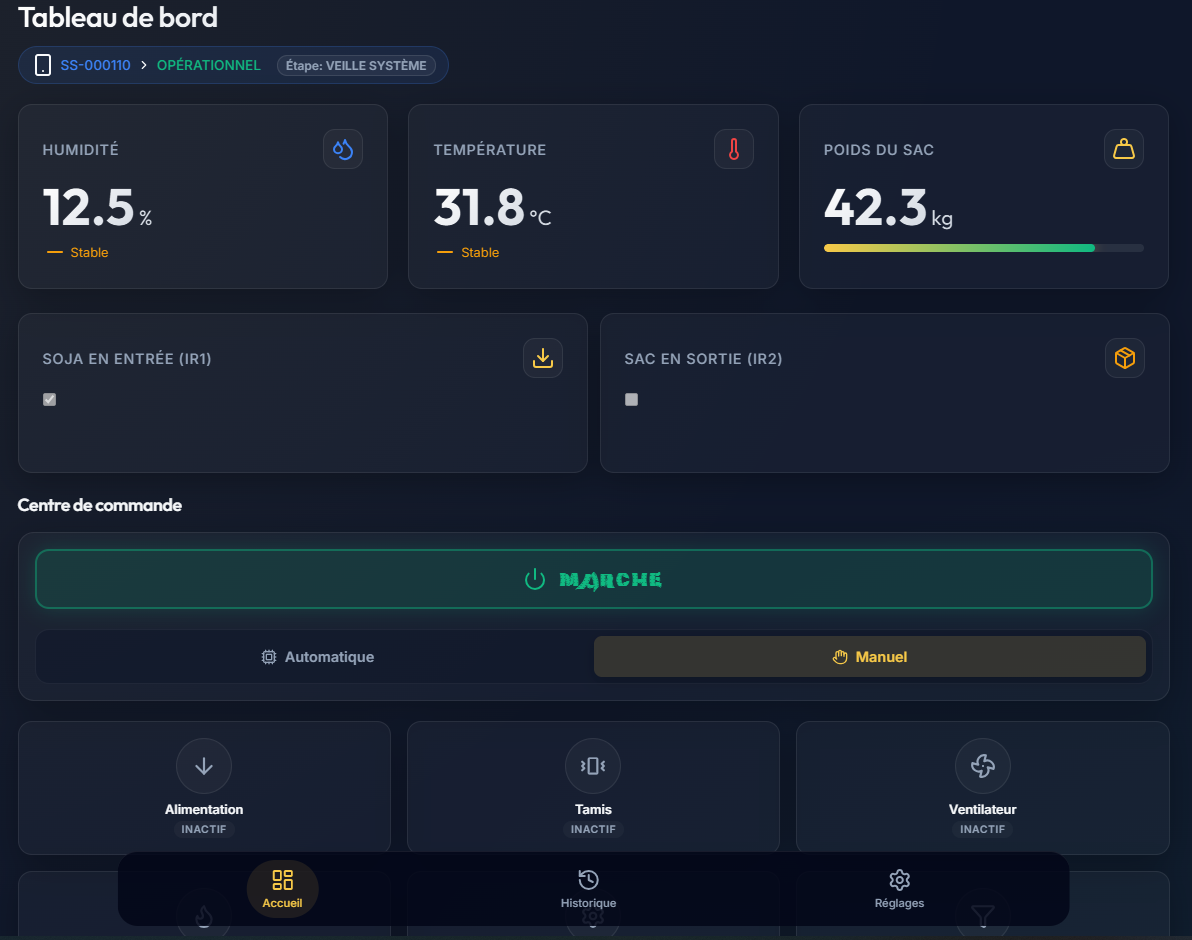
\includegraphics[width=\textwidth]{images/dashboard_producteur.png}
        \caption{Tableau de bord de supervision}
        \label{fig:iot_exploitant_dashboard}
    \end{subfigure}
    \hfill
    \begin{subfigure}[b]{0.49\textwidth}
        \centering
        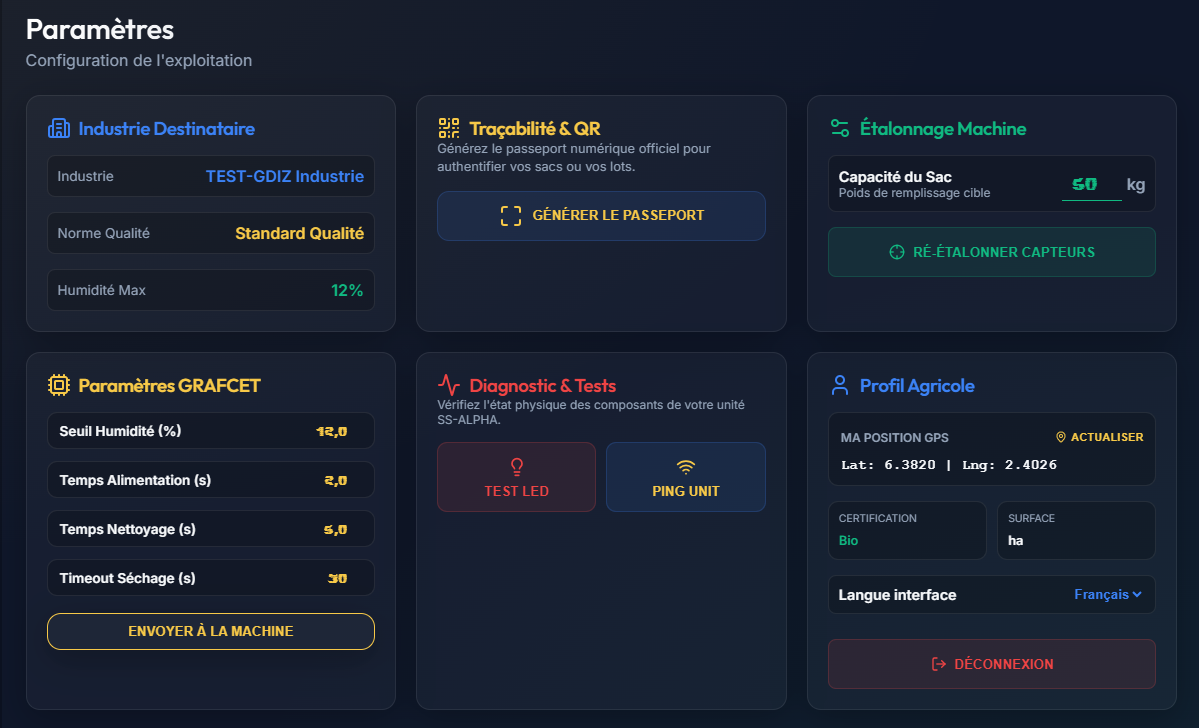
\includegraphics[width=\textwidth]{images/image_config_producteur.png}
        \caption{Interface de configuration}
        \label{fig:iot_exploitant_config}
    \end{subfigure}
    \caption{Supervision en temps réel et configuration des paramètres}
    \label{fig:iot_interfaces_ensemble}
\end{figure}
\FloatBarrier

\begin{figure}[H]
    \centering
    \begin{subfigure}[b]{0.49\textwidth}
        \centering
        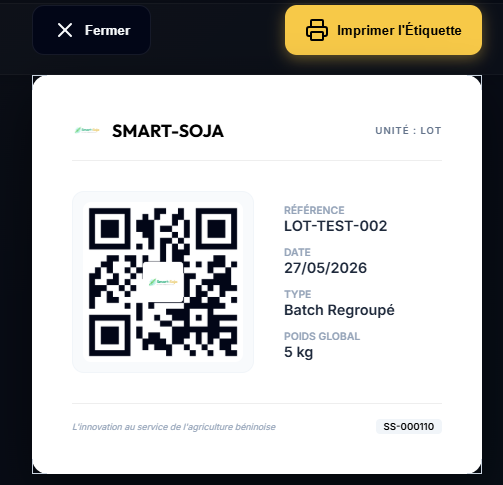
\includegraphics[width=\textwidth]{images/image_codeQR_genere.png}
        \caption{Étiquette de lot et QR Code}
        \label{fig:iot_etiquette_qr}
    \end{subfigure}
    \hfill
    \begin{subfigure}[b]{0.49\textwidth}
        \centering
        
\includegraphics[width=\textwidth]{images/image_doc_tracabilite.png}
        \caption{Certificat et passeport numérique}
        \label{fig:iot_certificat}
    \end{subfigure}
    \caption{Documents générés et certification de traçabilité}
    \label{fig:iot_documents_ensemble}
\end{figure}
\FloatBarrier

\textbf{Conclusion :} L'ensemble de la chaîne documentaire fonctionne. Les opérateurs accèdent facilement aux données via le tableau de bord, et les certificats générés sont clairs et utilisables pour la traçabilité commerciale.

% -------------------------------------------------------
\section{Synthèse d'état : résultats de validation fonctionnelle}
% -------------------------------------------------------

Le Tableau~\ref{tab:synthese_etat} résume l'état opérationnel de chaque fonction du prototype en distinguant clairement ce qui a été démontré en fonctionnement de ce qui reste à évaluer en charge réelle.

\begin{table}[H]
    \caption{État de validation fonctionnelle des sous-systèmes}
    \label{tab:synthese_etat}
    \centering
\small
\renewcommand{\arraystretch}{1.5}
\rowcolors{2}{white}{lightGray}
\begin{tabularx}{\textwidth}{|p{1.5cm}|L|p{2.2cm}|C|}
\hline
\rowcolor{lightGray}
\textbf{Fonction} & \textbf{Fonctionnalité testée} & \textbf{Validation} & \textbf{Statut} \\ \hline
Moteur tamis & Rotation continue, vibration & Observation directe + multimètre & \textcolor{green!60!black}{\textbf{Opérationnel}} \\ \hline
Capteur DHT22 & Affichage T°C et HR en temps réel & Démontré en labo, variations cohérentes & \textcolor{green!60!black}{\textbf{Opérationnel}} \\ \hline
Sondes d'humidité & Variation cohérente avec état soja & Démontré avec soja test & \textcolor{green!60!black}{\textbf{Opérationnel}} \\ \hline
Résistance chauffante & Chauffe observable + consommation & Mesure multimètre et thermique visuelle & \textcolor{green!60!black}{\textbf{Opérationnel}} \\ \hline
Ventilateur & Circulation d'air & Observation directe & \textcolor{green!60!black}{\textbf{Opérationnel}} \\ \hline
Interface LCD & Affichage des valeurs en temps réel & Démonstration directe & \textcolor{green!60!black}{\textbf{Opérationnel}} \\ \hline
Transmission MQTT & Envoi et réception des données & Test en labo avec broker public & \textcolor{green!60!black}{\textbf{Opérationnel}} \\ \hline
\end{tabularx}
\end{table}

\textbf{Synthèse :} Tous les sous-systèmes ont été validés en fonctionnement individuel et en intégration partielle. La chaîne complète (acquisition -- traitement -- affichage -- transmission) est opérationnelle.

% -------------------------------------------------------
\section{Discussion : résultats obtenus et limitations}
% -------------------------------------------------------

\subsection{Synthèse des validations fonctionnelles réalisées}

La validation du prototype SMART-SOJA a démontré le fonctionnement correct de l'ensemble de la chaîne système :

\begin{enumerate}
    \item \textbf{Acquisition de données :} Le capteur DHT22 fournit des mesures stables de température et humidité relative. Les sondes capacitives répondent cohéremment à l'état d'humidité du soja. L'interface LCD affiche l'ensemble des paramètres en temps réel.
    
    \item \textbf{Traitement et pilotage :} Le microcontrôleur ESP32 exécute correctement la logique de contrôle : allumage/extinction des actionneurs, gestion de l'interface, sauvegarde des données en local.
    
    \item \textbf{Actionneurs :} Le moteur du tamis tourne et provoque l'oscillation attendue du cadre de tamisage. La résistance chauffante produit la chaleur observable. Le ventilateur crée un flux d'air. Les servomoteurs répondent aux commandes.
    
    \item \textbf{Traçabilité numérique :} La génération de QR Code et la transmission des données par MQTT fonctionnent correctement. Les payloads JSON sont reçus sans erreur sur le broker.
    
    \item \textbf{Fiabilité :} L'arrêt d'urgence répond instantanément. Le système de sauvegarde locale enregistre les données en cas de déconnexion réseau.
\end{enumerate}

\subsection{Limitations de la validation actuelle}

Cette validation fonctionnelle reste partielle sur plusieurs points importants :

\begin{itemize}
    \item \textbf{Cycle complet nettoyage + séchage :} Le prototype a été testé composant par composant, mais pas en cycle opérationnel complet prolongé. La performance globale du nettoyage (taux de pureté) et du séchage (atteinte du seuil d'humidité cible) n'a pas été quantifiée précisément.
    
    \item \textbf{Charge réelle :} Les tests ont porté sur des petites masses de soja de test. Le comportement en charge réelle (charges de 2 à 5~kg) pourrait différer.
    
    \item \textbf{Conditions environnementales extrêmes :} Les tests ont été réalisés en laboratoire stable. La robustesse en conditions de terrain (poussière, vibrations, chaleur intense) reste à valider.
    
    \item \textbf{Autonomie réelle :} L'estimation d'autonomie repose sur les mesures de courant isolé de chaque sous-système. L'autonomie réelle dépendra du cycle opérationnel exact adopté en utilisation.
    
    \item \textbf{Module de pesée (HX711) :} La validation de la précision et de la stabilité du module de pesée (cellule de charge HX711) sera réalisée lors d'une phase d'intégration ultérieure, après finalisation des autres sous-systèmes critiques.
\end{itemize}

\subsection{Recommandations pour amélioration et tests complémentaires}

Les améliorations et tests prioritaires avant déploiement opérationnel en conditions réelles sont :

\begin{enumerate}
    \item \textbf{Validation du cycle opérationnel complet :} Réaliser des cycles complets nettoyage + séchage avec charges progressives (100~g, 500~g, 2~kg, 5~kg) en conditions de laboratoire. Mesurer précisément : (i) le temps de séchage pour atteindre une cible d'humidité définie, (ii) le taux de pureté du soja après tamisage, (iii) la stabilité de la température et de l'humidité dans la chambre de séchage.
    
    \item \textbf{Intégration du module de pesée (HX711) :} Procéder à l'acquisition et l'intégration du capteur de poids et du module HX711. Valider la précision du système de pesée sur la plage 0--5~kg et l'étalonnage du capteur selon le cahier des charges.
    
    \item \textbf{Validation énergétique en charge réelle :} Mesurer l'autonomie réelle de la batterie lors de cycles complets. Identifier les appels de courant pic en charge et vérifier la stabilité thermique de l'électronique sous fonctionnement prolongé.
    
    \item \textbf{Tests de robustesse mécanique :} Valider la résistance du cadre de tamisage à vibrations prolongées (> 30 minutes) et identifier les points d'usure ou les renforts structurels nécessaires.
    
    \item \textbf{Protocole de maintenance et opérationnel :} Documenter complètement la maintenance préventive (nettoyage des tamis, inspection des connexions, étalonnage périodique des capteurs) et réaliser des fiches techniques pour l'opérateur.
    
    \item \textbf{Tests en conditions environnementales de terrain :} Une fois les étapes précédentes validées, tester le prototype en conditions extérieures (variations de température > 30~°C, humidité relative > 70~\%, exposition à la poussière) pour valider la robustesse en conditions d'utilisation réelle.
\end{enumerate}

% -------------------------------------------------------
\section{Tableau d'évaluation financière}
% -------------------------------------------------------

Le tableau~\ref{tab:evaluation_financiere} présente le détail des dépenses engagées pour la conception et la réalisation du prototype SMART-SOJA. Les prix sont exprimés en francs CFA (FCFA), relevés auprès des fournisseurs locaux de Cotonou.

\begin{longtable}{|p{7.2cm}|c|c|c|}
\caption{Tableau d'évaluation financière du prototype (en FCFA)} \label{tab:evaluation_financiere} \\
\hline
\rowcolor{lightGray}
\textbf{Désignation} &
\textbf{Qté} &
\textbf{P.U. (FCFA)} &
\textbf{Total (FCFA)} \\ \hline
\endfirsthead
\hline
\rowcolor{lightGray}
\textbf{Désignation} &
\textbf{Qté} &
\textbf{P.U. (FCFA)} &
\textbf{Total (FCFA)} \\ \hline
\endhead
\hline
\endfoot
\hline
\endlastfoot

Écran LCD 16×2 avec interface I2C & 1 & 3~270 & 3~270 \\ \hline
Capteur DHT22 (température \& humidité) & 1 & 4~500 & 4~500 \\ \hline
Sonde capacitive d'humidité du sol & 2 & 300 & 600 \\ \hline
Module lecteur Carte SD & 1 & 2~600 & 2~600 \\ \hline
Régulateur LM2596 & 1 & 1~610 & 1~610 \\ \hline
Moteur JGA25-370 & 2 & 3~400 & 6~800 \\ \hline
Servomoteur SG90 & 2 & 1~400 & 2~800 \\ \hline
Transistor BC547 & 1 & 70 & 70 \\ \hline
Ventilateur 12~V DC & 2 & 2~000 & 4~000 \\ \hline
Résistance chauffante 12~V & 2 & 1~400 & 2~800 \\ \hline
MOSFET IRLZ44N & 4 & 500 & 2~000 \\ \hline
Fusible 5~A & 1 & 200 & 200 \\ \hline
Prise Jack d'alimentation & 2 & 150 & 300 \\ \hline
Bouton poussoir & 2 & 100 & 200 \\ \hline
Potentiomètre rotatif & 2 & 482 & 964 \\ \hline
Bouton potentiomètre & 2 & 100 & 200 \\ \hline
LED (Rouge/Vert/Bleu) & 12 & 21 & 252 \\ \hline
Résistance 10~k$\Omega$ & 12 & 20 & 240 \\ \hline
Résistance 4,7~k$\Omega$ & 4 & 20 & 80 \\ \hline
Résistance 1~k$\Omega$ & 4 & 20 & 80 \\ \hline
Résistance 220~$\Omega$ & 6 & 20 & 120 \\ \hline
Diode 1N5408 & 8 & 75 & 600 \\ \hline
Condensateur 100~nF & 10 & 150 & 1~500 \\ \hline
Condensateur 470~µF & 6 & 150 & 900 \\ \hline
Condensateur 10~µF & 4 & 150 & 600 \\ \hline
Condensateur 100~µF & 2 & 144 & 288 \\ \hline
Condensateur 1~000~µF & 1 & 250 & 250 \\ \hline
Bornier à vis 2 contacts & 10 & 145 & 1~450 \\ \hline
Barrette de pins mâles & 3 & 300 & 900 \\ \hline
Barrette de pins femelles & 3 & 300 & 900 \\ \hline
Jumper M/F & 20 & 35 & 700 \\ \hline
Jumper M/M & 20 & 35 & 700 \\ \hline
Impression PCB (double face, Cotonou) & 1 & 9~720 & 9~720 \\ \hline
Contre-platé (châssis) & 2 & 5~300 & 10~600 \\ \hline
Tuyau carré 30×30~mm & 3 & 5~000 & 15~000 \\ \hline
Baguette de bois & 1 & 500 & 500 \\ \hline
Lame de scie & 1 & 500 & 500 \\ \hline
Tamis vibrant & 2 & 1~300 & 2~600 \\ \hline
Graines de soja & 5~kg & 400 & 2~000 \\ \hline
Peinture et apprêt du châssis & 1 & 5~000 & 5~000 \\ \hline
Main d'œuvre soudeur (Châssis) & 1 & 5~000 & 5~000 \\ \hline
Roulement & 5 & 400 & 2~000 \\ \hline
\rowcolor{lightGray}
\multicolumn{3}{|r|}{\textbf{TOTAL GÉNÉRAL}} & \textbf{102~894} \\
\end{longtable}

\section*{Synthèse et transition}
Ce chapitre a présenté la validation fonctionnelle du prototype SMART-SOJA à travers des tests unitaires rigoureux et une démonstration complète de la chaîne numérique de traçabilité. L'ensemble des sous-systèmes testés — acquisition de données, tamisage, séchage, alimentation énergétique et transmission Internet des objets — s'est révélé opérationnel, tout en mettant en évidence des limitations, notamment sur la charge réelle, le cycle complet nettoyage-séchage et l'intégration du module de pesée, qui définissent les priorités des travaux futurs. Ces résultats, replacés dans la perspective du bilan financier du prototype, permettent de dresser le bilan global du projet SMART-SOJA et d'en dégager les perspectives de développement, objets de la conclusion générale.
